\documentclass{beamer}

% Theme choice
\usetheme{Madrid}

% Packages
\usepackage{graphicx} % For including images
\usepackage{amsmath} % For math equations
\usepackage{hyperref} % For hyperlinks

% Title details
\titlegraphic{
\includegraphics[width=4cm]{images/college-logo.png}}
\title[Alternate Assessment Test]{Design of EEG P300 Wave Detection using Verilog} 
\author{Arundhati, Karthik M Dani, Sanjana WG}
\institute{Department of Medical Electronics Engineering, \newline BMS College of Engineering, Bangalore} 
\date{\today}


\begin{document}

% Title Slide
\begin{frame}
    \titlepage
\end{frame}

% Outline Slide
\begin{frame}{Outline}
    \tableofcontents
\end{frame}

% Section: Introduction
% What is EEG
\section{Introduction}
\begin{frame}{What is EEG?}
\begin{itemize}

\item \textbf{Electroencephalography (EEG)} Measurement of voltage fluctuations caused by neural activity.
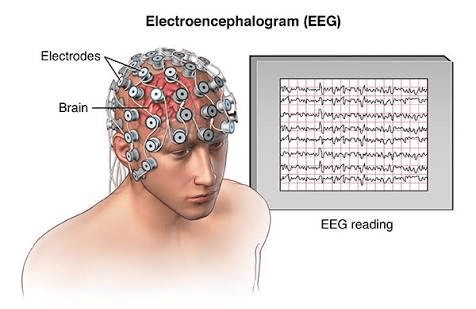
\includegraphics[width=0.6\linewidth]{images/eeg.png}
        
\end{itemize}
\end{frame}

% P300 Wave
\begin{frame}{What is P300 Wave?}
\begin{itemize}

\item P300 wave is a \textbf{ParietoCentral} Positive Deflection in Human Event-Related Potential (ERP), with a typical \textbf{latency of 300 milliseconds} after a stimulus. 

\item It is associated with attention and decision-making processes.

\item A Measure of \textbf{Cognitive Ability}.

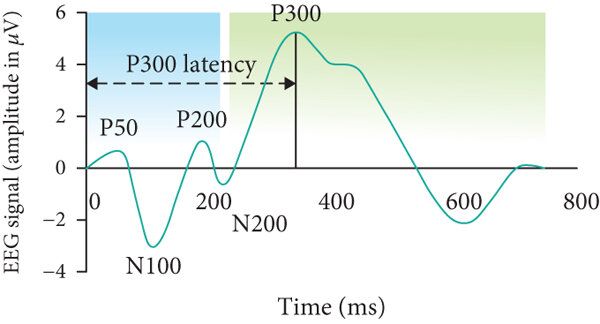
\includegraphics[width=0.8\linewidth]{images/P300-Waveform.png}

\end{itemize}
\end{frame}

\begin{frame}{What is P300 Wave?}
\begin{itemize}

\item \textbf{Objective of the Project:} 
\begin{itemize}
\item Design and implement a system capable of real-time detection of the P300 wave pattern using Verilog.
\end{itemize}
\item \textbf{Applications of P300 Detection:}
\begin{itemize}
\item Brain-Computer Interfaces (BCIs) for assistive technologies.
\item Neuropsychological studies related to attention and memory.
\item Diagnosing and monitoring neurological conditions.
\end{itemize}

\end{itemize}
\end{frame}

% Section 2: Problem Statement (Presenter 1)
\section{Problem Statement}
\begin{frame}{Problem Statement}
    \begin{block}{Core Question}
        What challenges does the traditional assessment method face?
    \end{block}
    \begin{itemize}
        \item Issues with inclusivity and accessibility
        \item Lack of flexibility in assessment methods
        \item Difficulty in assessing applied knowledge
    \end{itemize}
\end{frame}

% Section 3: Methodology (Presenter 2)
\section{Methodology}
\begin{frame}{Methodology}
    \textbf{Presenter 2}
    \begin{enumerate}
        \item Define clear learning outcomes
        \item Develop assessment rubrics
        \item Integrate project-based evaluation
        \item Provide feedback loops for improvement
    \end{enumerate}
\end{frame}

% Section 4: Results & Analysis (Presenter 2)
\section{Results and Analysis}
\begin{frame}{Results and Analysis}
    \textbf{Presenter 2}
    \begin{itemize}
        \item Increased student engagement and understanding
        \item Greater alignment of assessments with real-world applications
        \item Enhanced fairness and transparency in evaluations
    \end{itemize}
    \begin{figure}
        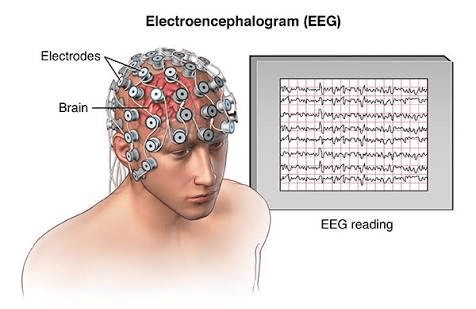
\includegraphics[width=0.8\linewidth]{images/eeg.png}
        \caption{Analysis of Assessment Outcomes}
    \end{figure}
\end{frame}

% Section 5: Conclusion and Recommendations (Presenter 3)
\section{Conclusion and Recommendations}
\begin{frame}{Conclusion}
    \textbf{Presenter 3}
    \begin{itemize}
        \item Summary of findings and implications
        \item Advantages of alternate assessment methods
        \item Future directions and recommendations
    \end{itemize}
\end{frame}

% Section 6: Final Slide (Presenter 3)
\begin{frame}{Questions?}
    \centering
    \Large Thank You! \\
    \vspace{1cm}
    \normalsize
    Questions are welcome.
\end{frame}

\end{document}